\section{Zachowanie robotów wewnątrz pola}
	Zachowanie robotów wewnątrz pola zamodelowane jest za pomocą metody sztucznych pól potencjałów. Potencjały ustalane są w następujący sposób:
	\begin{itemize}
		\item robot oczekujący na zezwolenie wyjazdu z pola widzi wszystkie ściany jako spolaryzowane ładunkiem o znaku zgodnym ze znakiem jego ładunku (rys. \ref{pic:waiting}), a jego wektor sił ma składowe opisane następującymi równaniami:
                  $$F_x= A*((X-x)^2 - x^2)$$
		  $$F_y= A*((Y-y)^2 - y^2),$$
		\item robot wykonujący manewr przejazdu do innego pola widzi dodatkowy ładunek na ścianie, w kierunku której ma zmierzać (umieszczony z jej prawej strony, aby zapobiegać kolizjom) (rys. \ref{pic:moving}), a do składowych jego wektora sił dodaje się człon odpowiedzialny za modelowanie dodatkowego potencjału:
                  $$F_{xM}= +\frac{B}{(X_p-x)^2}$$
                  $$F_{yM}= +\frac{B}{(Y_p-y)^2},$$
		\item dwa roboty znajdujące się w tym samym polu zawsze są spolaryzowane ładunkami punktowymi o jednakowych znakach (rys. \ref{pic:tworobots}), a do wektora sił dodawany jest w tym wypadku następujący człon modelujący siłę wzajemnie je odpychającą:
                  $$F_{xD}= +\frac{C}{\mathrm{sgn}(x-x_D)(x-x_D)^2}$$
                  $$F_{yD}= +\frac{C}{\mathrm{sgn}(y-y_D)(y-y_D)^2},$$ 
		\item w wypadku, jeśli w polu znajdują się dwa roboty, każdy widzi inną polaryzację ścian -- taką, aby zgadzała się ona z jego stanem ruchu (oczekiwanie, zezwolenie na przejazd),
                \item przykład --- kiedy w polu znajdują się dwa roboty i robot, dla którego obliczamy wypadkowy wektor sił, wyjeżdża z pola, składowe jego sił opisane są nastepującymi równaniami:
                  $$F_x= A((X-x)^2 - x^2)+B(X_p-x)^2+C(x-x_D)^2$$
                  $$F_y= A((Y-y)^2 - y^2)+B(Y_p-y)^2+C(y-y_D)^2.$$ 
	\end{itemize}
	
	\begin{figure}[H]
		\centering
		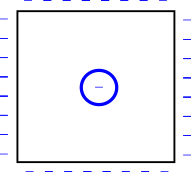
\includegraphics[scale=0.9]{img/waiting.png}
		\caption{Robot oczekujący na pozwolenie na wyjazd z komórki}
		\label{pic:waiting}
	\end{figure}
	\begin{figure}[H]
		\centering
		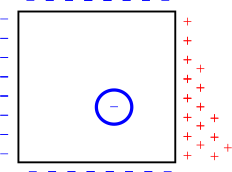
\includegraphics[scale=0.9]{img/moving.png}
		\caption{Robot wyjeżdżający z komórki}
		\label{pic:moving}
	\end{figure}
	\begin{figure}[H]
		\centering
		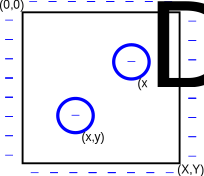
\includegraphics[scale=0.9]{img/tworobots.png}
		\caption{Dwa roboty oczekujące na pozwolenie na wyjazd z pola}
		\label{pic:tworobots}
	\end{figure}
